\documentclass[tikz,border=6mm]{standalone}
\usepackage{tikz}
\usepackage{xcolor}
\usetikzlibrary{arrows.meta,calc,decorations.pathmorphing,decorations.markings,shapes.geometric,positioning,backgrounds,fit,shadings,patterns}
\definecolor{substblue}{RGB}{70,130,180}
\definecolor{procamber}{RGB}{180,110,30}
\definecolor{feltgreen}{RGB}{0,110,55}
\definecolor{bgcream}{RGB}{252,248,240}
\definecolor{atomblue}{RGB}{100,160,210}
\definecolor{emphred}{RGB}{160,40,40}
\definecolor{panelborder}{RGB}{180,170,155}

\begin{document}
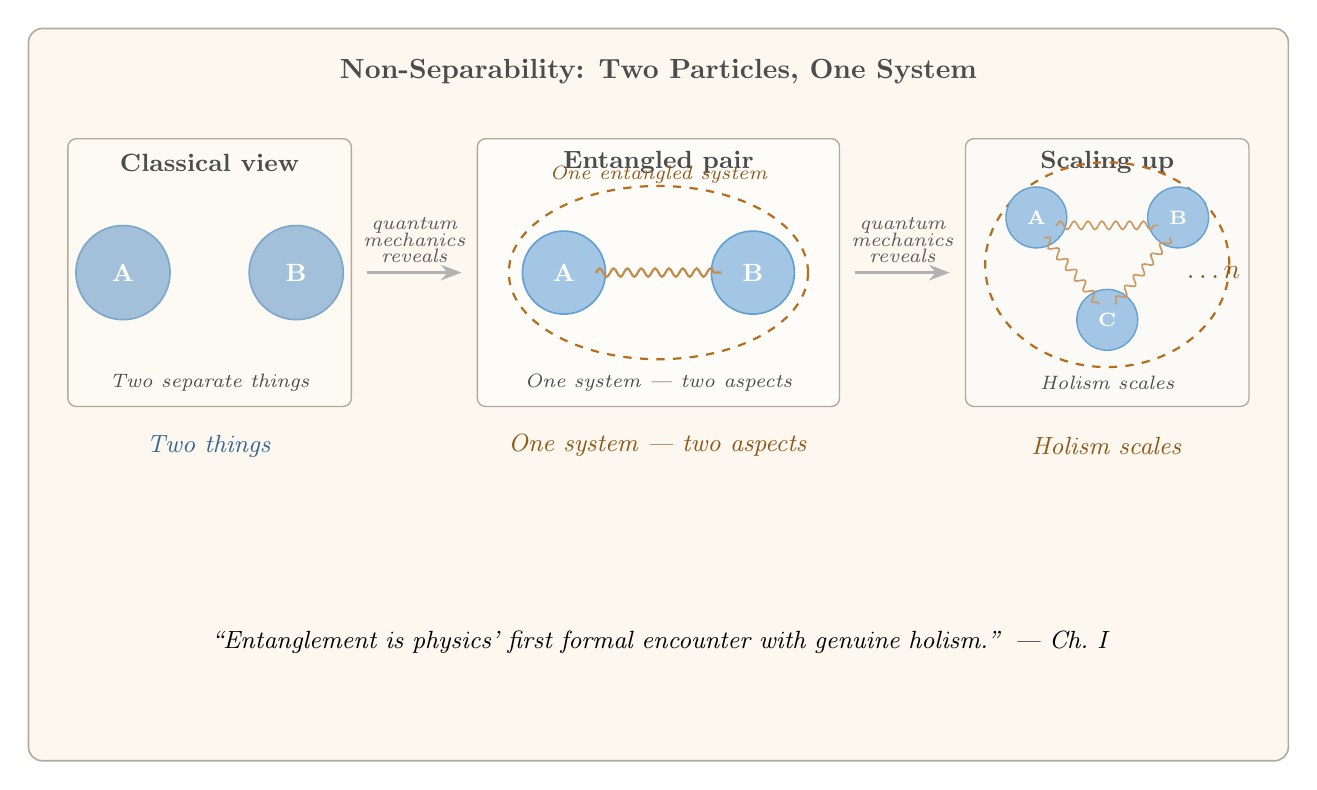
\begin{tikzpicture}[>=Stealth,font=\small,
  wavy/.style={decorate,decoration={snake,amplitude=1.5pt,segment length=5pt}}]

%% ── outer background ─────────────────────────────────────────────────────────
\fill[bgcream,rounded corners=5pt] (-0.5,-4.5) rectangle (15.5,4.8);
\draw[panelborder,rounded corners=5pt,line width=0.6pt]
  (-0.5,-4.5) rectangle (15.5,4.8);

%% ── title ────────────────────────────────────────────────────────────────────
\node[font=\normalsize\bfseries,gray!60!black] at (7.5,4.25)
  {Non-Separability: Two Particles, One System};

%% ════════════════════════════════════════════════════════════════════════════
%%  LEFT PANEL — Classical view
%% ════════════════════════════════════════════════════════════════════════════
\fill[bgcream!80!white,rounded corners=3pt] (0.0,0.0) rectangle (3.6,3.4);
\draw[panelborder,rounded corners=3pt,line width=0.5pt] (0.0,0.0) rectangle (3.6,3.4);

\node[font=\small\bfseries,gray!60!black,align=center]
  at (1.8,3.1) {Classical view};

%% two separate circles, far apart
\fill[substblue!50] (0.7,1.7) circle (17pt);
\draw[substblue!70,line width=0.6pt] (0.7,1.7) circle (17pt);
\node[font=\bfseries\small,white] at (0.7,1.7) {A};

\fill[substblue!50] (2.9,1.7) circle (17pt);
\draw[substblue!70,line width=0.6pt] (2.9,1.7) circle (17pt);
\node[font=\bfseries\small,white] at (2.9,1.7) {B};

%% no connection
\node[font=\scriptsize\itshape,gray!60!black,align=center] at (1.8,0.3)
  {Two separate things};

%% ── transition arrow 1 ───────────────────────────────────────────────────────
\draw[->,gray!60,line width=1.0pt] (3.8,1.7) -- (5.0,1.7);
\node[above,font=\scriptsize\itshape,gray!70!black,align=center,text width=1.8cm]
  at (4.4,1.7) {quantum\\[-2pt]mechanics\\[-2pt]reveals};

%% ════════════════════════════════════════════════════════════════════════════
%%  MIDDLE PANEL — Entangled pair
%% ════════════════════════════════════════════════════════════════════════════
\fill[bgcream!80!procamber!10,rounded corners=3pt] (5.2,0.0) rectangle (9.8,3.4);
\draw[panelborder,rounded corners=3pt,line width=0.5pt] (5.2,0.0) rectangle (9.8,3.4);

\node[font=\small\bfseries,gray!60!black] at (7.5,3.1) {Entangled pair};

%% dashed oval enclosing both
\draw[procamber,thick,dashed] (7.5,1.7) ellipse (1.9cm and 1.1cm);

%% two circles inside
\fill[atomblue!60] (6.3,1.7) circle (15pt);
\draw[atomblue,line width=0.6pt] (6.3,1.7) circle (15pt);
\node[font=\bfseries\small,white] at (6.3,1.7) {A};

\fill[atomblue!60] (8.7,1.7) circle (15pt);
\draw[atomblue,line width=0.6pt] (8.7,1.7) circle (15pt);
\node[font=\bfseries\small,white] at (8.7,1.7) {B};

%% wavy line between
\draw[procamber!80,line width=0.8pt,wavy] (6.7,1.7) -- (8.3,1.7);

%% oval label
\node[procamber!80!black,font=\scriptsize\itshape,align=center]
  at (7.5,2.95) {One entangled system};

\node[font=\scriptsize\itshape,gray!60!black,align=center] at (7.5,0.3)
  {One system --- two aspects};

%% ── transition arrow 2 ───────────────────────────────────────────────────────
\draw[->,gray!60,line width=1.0pt] (10.0,1.7) -- (11.2,1.7);
\node[above,font=\scriptsize\itshape,gray!70!black,align=center,text width=1.8cm]
  at (10.6,1.7) {quantum\\[-2pt]mechanics\\[-2pt]reveals};

%% ════════════════════════════════════════════════════════════════════════════
%%  RIGHT PANEL — Scaling up
%% ════════════════════════════════════════════════════════════════════════════
\fill[bgcream!80!procamber!15,rounded corners=3pt] (11.4,0.0) rectangle (15.0,3.4);
\draw[panelborder,rounded corners=3pt,line width=0.5pt] (11.4,0.0) rectangle (15.0,3.4);

\node[font=\small\bfseries,gray!60!black] at (13.2,3.1) {Scaling up};

%% larger dashed oval
\draw[procamber,thick,dashed] (13.2,1.8) ellipse (1.55cm and 1.3cm);

%% three circles in a triangle arrangement
\fill[atomblue!60] (12.3,2.4) circle (11pt);
\draw[atomblue,line width=0.5pt] (12.3,2.4) circle (11pt);
\node[font=\bfseries\scriptsize,white] at (12.3,2.4) {A};

\fill[atomblue!60] (14.1,2.4) circle (11pt);
\draw[atomblue,line width=0.5pt] (14.1,2.4) circle (11pt);
\node[font=\bfseries\scriptsize,white] at (14.1,2.4) {B};

\fill[atomblue!60] (13.2,1.1) circle (11pt);
\draw[atomblue,line width=0.5pt] (13.2,1.1) circle (11pt);
\node[font=\bfseries\scriptsize,white] at (13.2,1.1) {C};

%% wavy lines among all three
\draw[procamber!70,line width=0.6pt,wavy] (12.55,2.3) -- (13.85,2.3);
\draw[procamber!70,line width=0.6pt,wavy] (12.4,2.15) -- (13.1,1.3);
\draw[procamber!70,line width=0.6pt,wavy] (14.0,2.15) -- (13.3,1.3);

%% ellipsis suggesting more
\node[font=\normalsize,procamber!80!black] at (14.55,1.7) {$\ldots n$};

\node[font=\scriptsize\itshape,gray!60!black,align=center] at (13.2,0.3)
  {Holism scales};

%% ── caption ──────────────────────────────────────────────────────────────────
\node[font=\small\itshape,text width=13cm,align=center]
  at (7.5,-3.0)
  {``Entanglement is physics' first formal encounter with genuine holism.'' --- Ch.~I};

%% ── sub-panel labels (below each panel) ──────────────────────────────────────
\node[font=\small,substblue!80!black,align=center] at (1.8,-0.5)
  {\small\textit{Two things}};
\node[font=\small,procamber!80!black,align=center] at (7.5,-0.5)
  {\small\textit{One system --- two aspects}};
\node[font=\small,procamber!80!black,align=center] at (13.2,-0.5)
  {\small\textit{Holism scales}};

\end{tikzpicture}
\end{document}
